\documentclass[11pt]{article}
\usepackage[margin=0.9in]{geometry}
\usepackage{mathptmx}
\usepackage{amsmath,amssymb,amsthm}
\usepackage{booktabs}
\usepackage{graphicx}
\usepackage{caption}
\usepackage[hidelinks]{hyperref}
\usepackage{microtype}
\usepackage{natbib}
\captionsetup{font=small,labelfont=bf}
\newtheorem{proposition}{Proposition}
\newtheorem*{remark}{Remark}
\setlength{\parskip}{3pt}

\title{\textbf{Inside the Fee Band: Why Takers Cannot Beat Kalshi\\and Who Profits Anyway}}
\author{Reed Ostrov\\ \small Denison University}
\date{\small November 2026}

\begin{document}
\maketitle

\begin{abstract}
\noindent
Prediction market prices on Kalshi are close to calibrated, but not exactly: low-priced contracts win less often than their prices imply, and high-priced contracts win more often. This paper asks whether that miscalibration can be exploited after fees. Kalshi charges takers $0.07\,P(1-P)$ per contract, a fee proportional to the variance of the contract's payoff. A simple model shows that this fee, plus half the bid-ask spread, defines a band around the true probability inside which mispricing persists but no strategy that conditions only on price earns a positive expected return as a taker. Because makers pay no fee on most series, the band is narrower for them, and equilibrium mispricing should sit inside the taker band but outside the maker band. Published evidence covering 72.1 million Kalshi trades matches both predictions. At 50 cents, taker fills were mispriced by 1.33 cents against a 1.75-cent fee, while makers earned $+1.12\%$ per trade. Efficiency varies by a factor of roughly 40 across categories, from finance (0.17-point maker-taker gap) to world events (7.32 points). Polymarket shows the same calibration pattern with taker fees 57\% to 100\% of Kalshi's, and none on geopolitics. The strong claim that no one can profit on Kalshi is false. The narrower claim, that public-information takers cannot profit in the long run, is supported.
\end{abstract}

\section{Introduction}

A binary contract that pays \$1 if an event occurs and trades at price $P$ is commonly read as a probability. If the market is calibrated, events priced at 16 cents occur 16\% of the time. Large recent datasets show that Kalshi and Polymarket are close to this ideal and deviate in a stable direction, the favorite-longshot bias first documented in horse racing \citep{griffith1949,thaler1988}: longshots are overpriced and favorites underpriced \citep{becker2026,burgi2026,le2026}.

A stable bias raises an obvious question: why is it not traded away? The answer proposed here is that the fee schedule makes most of it untradeable for takers. The paper contributes three things. First, it formalizes a no-trade band implied by Kalshi's fee formula and shows the band differs by trader role. Second, it converts published calibration figures into net-of-fee returns. Third, it ranks market categories by efficiency and identifies where the band is narrowest relative to the bias. No new trade data are collected; all empirical inputs come from the cited studies and the platforms' published fee schedules.

\section{Institutional setting}

Kalshi's general fee for an order of $C$ contracts at price $P$ (in dollars) is $\lceil 0.07\,C\,P(1-P)\rceil$, rounded up to the cent, with a series multiplier that defaults to 1 \citep{kalshifees}. Resting (maker) orders pay nothing except on roughly 157 listed series, where the maker rate is 0.0175. There is no settlement fee. Kalshi also pays a variable 3.50\% annual rate on cash and open positions for balances of at least \$250 \citep{kalshiapy}.

Polymarket has used the same functional form since March 30, 2026, $C \cdot r \cdot P(1-P)$, with a category rate $r$: 0.07 for crypto, 0.05 for sports, economics, culture and weather, 0.04 for politics, finance and technology, and 0 for geopolitics \citep{polyfees}. Makers pay nothing and receive 15\% to 25\% of taker fees as rebates.

Table~\ref{tab:fees} shows the break-even win rate a Kalshi taker needs at each price, before the spread. Rounding matters for small orders: one contract at 50 cents is charged 2 cents and one contract at 95 cents is charged 1 cent, three times the formula value.

\begin{table}[h]
\centering\small
\caption{Kalshi taker fee and break-even probability, by price (formula value, before spread).}
\label{tab:fees}
\begin{tabular}{rrrr}
\toprule
Price & Fee per contract & Fee / cost & Required win rate \\
\midrule
1\textcent  & 0.07\textcent & 6.9\% & 1.07\% \\
5\textcent  & 0.33\textcent & 6.7\% & 5.33\% \\
16\textcent & 0.94\textcent & 5.9\% & 16.94\% \\
50\textcent & 1.75\textcent & 3.5\% & 51.75\% \\
84\textcent & 0.94\textcent & 1.1\% & 84.94\% \\
95\textcent & 0.33\textcent & 0.35\% & 95.33\% \\
\bottomrule
\end{tabular}
\end{table}

\section{A no-trade band}

Let $q$ be the true probability, $P$ the traded price, $s$ the bid-ask spread, and $\phi_j(P)=k_j P(1-P)$ the fee for role $j$, with $k_T = 0.07$ for takers and $k_M=0$ for makers on standard series. A taker who buys YES earns, per contract,
\begin{equation}
\pi_T = q - P - k_T P(1-P) - \tfrac{s}{2}.
\end{equation}
Buying NO gives the mirror image. Define the taker band $B_T(P)=k_T P(1-P)+s/2$.

\begin{proposition}[No-trade band]
If $|E[q\mid P]-P| \le B_T(P)$, no taker strategy that conditions only on $P$ has positive expected profit.
\end{proposition}

\begin{proposition}[Long-run bound]
Suppose the bias is public and arbitrageurs with price impact can enter freely. Then deviations outside $B_T$ attract taker flow that moves prices toward $q$ until the deviation is inside $B_T$. In steady state, $|E[q\mid P]-P| \le B_T(P)$ for public-information takers.
\end{proposition}

The bound is a version of \citet{grossman1980}: prices cannot be fully efficient, because someone must be paid to correct them. Here the payment is set by the fee schedule. Because $k_M < k_T$, the maker band $B_M$ is narrower than $B_T$. Mispricing that survives inside $B_T$ but exceeds $B_M$ is profitable to makers. The model therefore predicts that persistent calibration error transfers wealth from takers to makers.

\begin{proposition}[Aggregate identity]
Trading among participants is zero-sum before costs. Summed over all traders, $\sum_i \pi_i = -F$, where $F$ is total fees collected. Interest paid by the exchange is outside this identity and is added to it.
\end{proposition}

\begin{remark}[Fees as a tax on variance]
The payoff of one contract has variance $q(1-q)\approx P(1-P)$, so Kalshi's taker fee equals 7\% of payoff variance at every price. The break-even edge per unit of standard deviation is $0.07\sqrt{P(1-P)}$, which peaks at 0.035 at 50 cents and falls to 0.015 at 5 or 95 cents. The fee is lightest, in risk-adjusted terms, at the extremes, which is where the observed bias is largest.
\end{remark}

\section{Evidence}

\paragraph{Calibration.} \citet{becker2026} analyzes 72.1 million Kalshi trades (\$18.26 billion, 2021 to November 2025). Contracts priced at 5 cents won 4.18\% of the time and contracts at 95 cents won 95.83\%. Takers earned $-1.12\%$ per trade before fees and makers $+1.12\%$; takers had negative excess returns at 80 of 99 price levels. \citet{burgi2026}, using over 300{,}000 contracts with each contract weighted equally, find average pre-fee returns of about $-20\%$, with takers losing about 32\% and makers about 10\%. The equal weighting puts heavy weight on cheap longshots, which explains the larger magnitudes. \citet{le2026}, using 292 million trades on both platforms, estimate logistic recalibration slopes, where 1 is perfect calibration and values above 1 mean prices are compressed toward 50\%. Slopes are near 1 within a day of resolution and rise to between 1.20 and 1.74 beyond a month in five of six categories. A Princeton thesis on 188{,}509 Polymarket markets finds an overall slope of 1.112 \citep{princeton2026}.

\paragraph{Net returns.} Table~\ref{tab:net} applies the fee formula to Becker's published win rates. Figure~\ref{fig:band} plots the same points against the taker band.

\begin{table}[h]
\centering\small
\caption{Taker returns after Kalshi's fee, computed from \citet{becker2026}. Rows marked ``all'' pool maker and taker fills, so a pure taker would do somewhat worse.}
\label{tab:net}
\begin{tabular}{lrrrr}
\toprule
Position & Before fee & Fee & After fee & After fee, \% of stake \\
\midrule
Buy YES at 1\textcent\ (taker)  & $-0.57$\textcent & 0.07\textcent & $-0.64$\textcent & $-60\%$ \\
Buy at 5\textcent\ (all)        & $-0.82$\textcent & 0.33\textcent & $-1.15$\textcent & $-22\%$ \\
Buy at 50\textcent\ (taker)     & $-1.33$\textcent & 1.75\textcent & $-3.08$\textcent & $-6\%$ \\
Buy at 95\textcent\ (all)       & $+0.83$\textcent & 0.33\textcent & $+0.50$\textcent & $+0.5\%$ \\
\bottomrule
\end{tabular}
\end{table}

\begin{figure}[h]
\centering
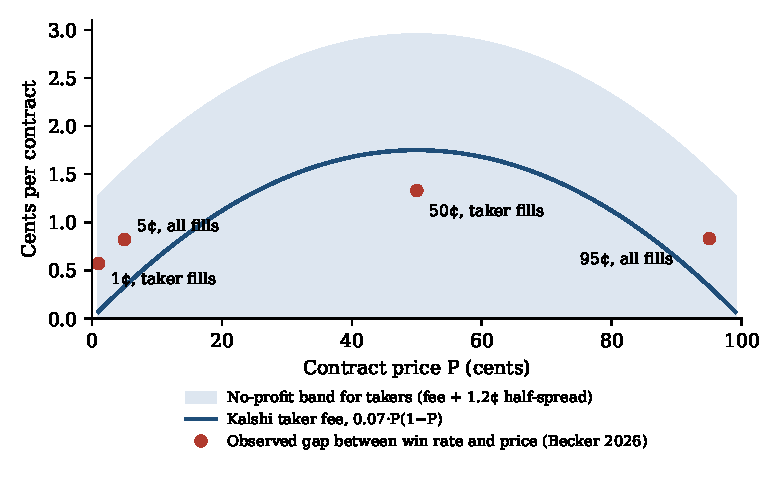
\includegraphics[width=0.68\linewidth]{fig1.pdf}
\caption{Kalshi's taker fee and the no-trade band (fee plus an assumed 1.2-cent half-spread), against observed mispricing at four prices. The half-spread follows a reported 2.4-cent median spread \citep{stockalarm} and is an assumption.}
\label{fig:band}
\end{figure}

At 50 cents, where most volume trades, the observed taker mispricing (1.33 cents) is smaller than the fee alone, as Proposition 2 predicts. At the extremes, the absolute bias is small but the fee is smaller still, so a thin positive margin appears for favorite buyers. That margin is statistically weak for any one trader. At 95 cents, a contract has an expected net gain of about 0.50 cents and a standard deviation of about 20 cents. Roughly 4{,}400 independent bets are needed before realized profit is positive with 95\% confidence, and correlated outcomes raise that number.

\paragraph{Categories.} Table~\ref{tab:cat} reports Becker's maker-taker gap by category, with Le's short-horizon slopes and Polymarket's fee for the comparable category.

\begin{table}[h]
\centering\small
\caption{Efficiency by category. Gap = maker return minus taker return per trade, before fees \citep{becker2026}. Slopes are the range over horizons under 24 hours \citep{le2026}.}
\label{tab:cat}
\begin{tabular}{lrrrrr}
\toprule
Category & Gap (pts) & Taker return & Trades & Slope, $<$24h & Polymarket fee at 50\textcent \\
\midrule
Finance       & 0.17 & $-0.08\%$ & 4.4M  & 0.96 to 1.07 & 1.00\textcent \\
Politics      & 1.02 & $-0.51\%$ & 4.9M  & 0.93 to 1.55 & 1.00\textcent \\
Sports        & 2.23 & $-1.11\%$ & 43.6M & 0.90 to 1.10 & 1.25\textcent \\
Weather       & 2.57 & $-1.29\%$ & 4.4M  & 0.69 to 0.91 & 1.25\textcent \\
Crypto        & 2.69 & $-1.34\%$ & 6.7M  & 0.99 to 1.07 & 1.75\textcent \\
Entertainment & 4.79 & $-2.40\%$ & 1.5M  & 0.81 to 1.02 & 1.25\textcent \\
Media         & 7.28 & $-3.64\%$ & 0.6M  & n.a.          & 1.00\textcent \\
World events  & 7.32 & $-3.66\%$ & 0.2M  & n.a.          & 0\textcent \\
\bottomrule
\end{tabular}
\end{table}

The ordering is consistent with participant selection. Finance questions attract traders who already price options and can anchor to futures; questions about sports, celebrities and world news attract participants whose sense of expertise is cheap to acquire. Weather is unusual: its short-horizon prices are too extreme (slopes below 1), the reverse of the usual bias. The least efficient category on Kalshi, world events, maps to the only fee-free category on Polymarket, so the band there shrinks to the spread. This is the strongest candidate for a taker edge, but Kalshi's estimate rests on only 0.2 million trades and the two platforms draw different traders.

\section{Discussion}

\paragraph{Who profits.} Three groups earn positive returns, and none relies on calibration alone. Makers earn the spread and the residual bias inside the taker band; Becker finds they have almost no directional skill (Cohen's $d \approx 0.02$). Informed takers profit from information the price does not yet contain: on Polymarket, \citet{gomezcram2026} classify about 3\% of 1.72 million accounts as skilled, 44\% of whom remain skilled out of sample, and market makers plus skilled takers capture over 30\% of gains. Favorite buyers earn a thin margin, as above.

\paragraph{Is the maker edge permanent?} Probably not. From 2021 to 2023, Kalshi takers outperformed makers by about 2 points; the sign reversed in late 2024 as quarterly volume rose from \$30 million to \$820 million and professional market makers entered \citep{becker2026}. Competition among makers should narrow $B_M$ profits in the same way taker competition bounds $B_T$.

\paragraph{Is the bias a mistake?} Not entirely. Long-horizon underpricing of favorites partly reflects capital lock-up: adjusting Polymarket prices for settlement discounting removes 48\% to 88\% of the horizon gradient \citep{gebele2026}. Kalshi's interest on open positions should shrink this component there. \citet{burgi2026} reproduce the pattern with a model in which takers are mildly over-optimistic about the contracts they buy. Under either reading, the mispricing is a price for something takers want, which explains why it persists.

\paragraph{Limitations.} First, contracts on the same event resolve together, so trade counts overstate independent observations; Le's strong political underconfidence (slopes up to 1.83) may reflect a few 2024 election outcomes, consistent with Becker's small political taker loss ($-0.51\%$). Second, the data end in late 2025, before Kalshi's February and July 2026 fee revisions and Polymarket's March 2026 fee expansion. Third, maker and taker labels proxy imperfectly for sophistication. Fourth, the 1.2-cent half-spread in Figure~\ref{fig:band} is an assumption.

\section{Conclusion}

The hypothesis that it is impossible to make money consistently on Kalshi is false in its strong form and supported in a narrower one. A taker who conditions only on public prices faces a fee proportional to payoff variance that exceeds observed miscalibration across most of the price range, and free entry should keep it that way. The surviving mispricing is a transfer from takers to makers, governed by the gap between their fee rates. A direct test of any proposed edge is to compute $q-P-0.07P(1-P)-s/2$ on out-of-sample resolved markets, counting events, not contracts, as observations.

\vspace{4pt}
\noindent{\small\textit{Disclosure.} This paper uses no proprietary data. Drafting was assisted by an AI model (Claude); all empirical figures are taken from or computed from the cited sources.}

\begin{thebibliography}{99}\small
\bibitem[Becker(2026)]{becker2026} Becker, J. (2026). The microstructure of wealth transfer in prediction markets. SSRN 7217640. \url{https://www.jbecker.dev/research/prediction-market-microstructure}
\bibitem[B\"urgi et~al.(2026)]{burgi2026} B\"urgi, C., Deng, W., \& Whelan, K. (2026). Makers and takers: The economics of the Kalshi prediction market. CEPR Discussion Paper 20631.
\bibitem[Gebele and Matthes(2026)]{gebele2026} Gebele, J., \& Matthes, F. (2026). When certainty is not worth it: Capital lock-up and settlement discounting in prediction markets. arXiv:2605.31431.
\bibitem[G\'omez-Cram et~al.(2026)]{gomezcram2026} G\'omez-Cram, R., Guo, Y., Jensen, T.~I., \& Kung, H. (2026). Prediction market accuracy: Crowd wisdom or informed minority? Working paper.
\bibitem[Griffith(1949)]{griffith1949} Griffith, R.~M. (1949). Odds adjustments by American horse-race bettors. \textit{American Journal of Psychology}, 62(2), 290-292.
\bibitem[Grossman and Stiglitz(1980)]{grossman1980} Grossman, S.~J., \& Stiglitz, J.~E. (1980). On the impossibility of informationally efficient markets. \textit{American Economic Review}, 70(3), 393-408.
\bibitem[Kalshi(2026a)]{kalshifees} Kalshi (2026a). Fee schedule, effective July 7, 2026. \url{https://kalshi.com/docs/kalshi-fee-schedule.pdf}
\bibitem[Kalshi(2026b)]{kalshiapy} Kalshi (2026b). Interest (APY) on Kalshi. Help center.
\bibitem[Le(2026)]{le2026} Le, N.~A. (2026). Decomposing crowd wisdom: Domain-specific calibration dynamics in prediction markets. arXiv:2602.19520.
\bibitem[Polymarket(2026)]{polyfees} Polymarket (2026). Fees. \url{https://docs.polymarket.com/trading/fees}
\bibitem[Princeton(2026)]{princeton2026} Anonymous (2026). The price is (almost) right: A calibration analysis of Polymarket pricing data. Senior thesis, Princeton University.
\bibitem[StockAlarm(2025)]{stockalarm} StockAlarm (2025). Prediction market analysis: 3,587 markets. \url{https://pro.stockalarm.io/blog/prediction-market-analysis}
\bibitem[Thaler and Ziemba(1988)]{thaler1988} Thaler, R.~H., \& Ziemba, W.~T. (1988). Anomalies: Parimutuel betting markets: Racetracks and lotteries. \textit{Journal of Economic Perspectives}, 2(2), 161-174.
\end{thebibliography}
\end{document}
